\chapter{Stakeholder Management}
\section{Stakeholder Identification}
\parindent20pt Stakeholders are classified based on their influence, interest, and level of engagement. Principal stakeholder groups encompass internal entities such as the CHSRA Executive Board, the Project Management Office, and the engineering and legal teams. Additionally, external stakeholders include the California State Legislature, the Federal Railroad Administration, local government authorities, landowners, environmental organizations, contractors, labor unions, community organizations, and the general public.

\section{Stakeholder Engagement Strategies}
The CHSRA deploys a tiered engagement plan: \par
\vspace*{0.2em}
\noindent 
\begin{center}
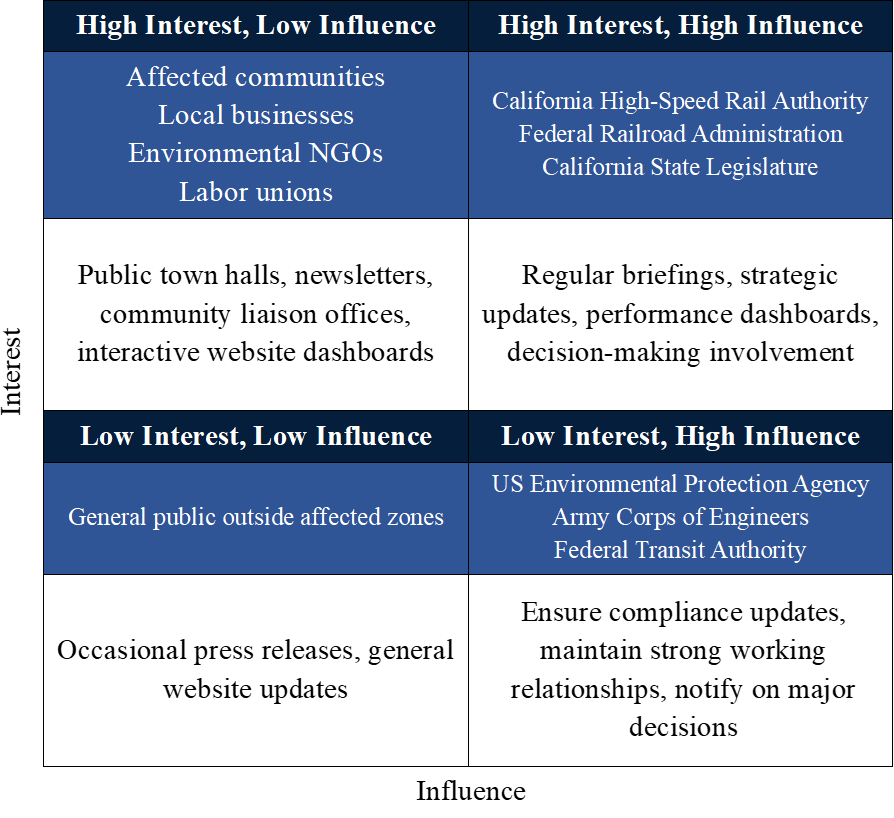
\includegraphics[width=\linewidth]{./attachments/lowhi}
\end{center}\par \justifying

\section{Stakeholder Communication Methods}
\parindent20pt Stakeholder communication is a vital part of any project. Guided by the Communications Management Plan, stakeholders can be informed through public engagement, regulatory reports, and community relations. Public engagement includes town halls, information sessions, and feedback surveys. Regulatory reports such as compliance reports, quarterly performance reviews, and lobbying updates also provide crucial statistics about the project. Community relations ensures that stakeholders are actively informed and kept happy. The CHSR authority established a Stakeholder Liaison Office to manage grassroots engagements, particularly concerning eminent domain and environmental disputes.

\section{Managing Conflicts and Resistance}
Resistance was expected, especially concerning land acquisition, environmental impact, and budget overruns. The Project Management Office applies conflict resolution strategies, including mediation and compensation mechanisms, along with mitigation techniques such as rerouting in sensitive areas and noise reduction measures. Additionally, targeted benefits are offered to impacted communities, such as employment opportunities. It also utilizes transparency tools, such as public dashboards and financial disclosures, notably the CHSR website, which has been effectively used as the primary source throughout this document. \par
